\documentclass[12pt,a4paper]{article}

%\usepackage[left=1.5cm,right=1.5cm,top=1cm,bottom=2cm]{geometry}
\usepackage[in, plain]{fullpage}
\usepackage{array}
\usepackage{../../../pas-math}
\usepackage{../../../moncours}


%\usepackage{pas-cours}
%-------------------------------------------------------------------------------
%          -Packages nécessaires pour écrire en Français et en UTF8-
%-------------------------------------------------------------------------------
\usepackage[utf8]{inputenc}
\usepackage[frenchb]{babel}
\usepackage[T1]{fontenc}
\usepackage{lmodern}
\usepackage{textcomp}



%-------------------------------------------------------------------------------

%-------------------------------------------------------------------------------
%                          -Outils de mise en forme-
%-------------------------------------------------------------------------------
\usepackage{hyperref}
\hypersetup{pdfstartview=XYZ}
%\usepackage{enumerate}
\usepackage{graphicx}
\usepackage{multicol}
\usepackage{tabularx}
\usepackage{multirow}


\usepackage{anysize} %%pour pouvoir mettre les marges qu'on veut
%\marginsize{2.5cm}{2.5cm}{2.5cm}{2.5cm}

\usepackage{indentfirst} %%pour que les premier paragraphes soient aussi indentés
\usepackage{verbatim}
\usepackage{enumitem}
\usepackage[usenames,dvipsnames,svgnames,table]{xcolor}

\usepackage{variations}

%-------------------------------------------------------------------------------


%-------------------------------------------------------------------------------
%                  -Nécessaires pour écrire des mathématiques-
%-------------------------------------------------------------------------------
\usepackage{amsfonts}
\usepackage{amssymb}
\usepackage{amsmath}
\usepackage{amsthm}
\usepackage{tikz}
\usepackage{xlop}
%-------------------------------------------------------------------------------



%-------------------------------------------------------------------------------


%-------------------------------------------------------------------------------
%                    - Mise en forme avancée
%-------------------------------------------------------------------------------

\usepackage{ifthen}
\usepackage{ifmtarg}


\newcommand{\ifTrue}[2]{\ifthenelse{\equal{#1}{true}}{#2}{$\qquad \qquad$}}

%-------------------------------------------------------------------------------

%-------------------------------------------------------------------------------
%                     -Mise en forme d'exercices-
%-------------------------------------------------------------------------------
%\newtheoremstyle{exostyle}
%{\topsep}% espace avant
%{\topsep}% espace apres
%{}% Police utilisee par le style de thm
%{}% Indentation (vide = aucune, \parindent = indentation paragraphe)
%{\bfseries}% Police du titre de thm
%{.}% Signe de ponctuation apres le titre du thm
%{ }% Espace apres le titre du thm (\newline = linebreak)
%{\thmname{#1}\thmnumber{ #2}\thmnote{. \normalfont{\textit{#3}}}}% composants du titre du thm : \thmname = nom du thm, \thmnumber = numéro du thm, \thmnote = sous-titre du thm

%\theoremstyle{exostyle}
%\newtheorem{exercice}{Exercice}
%
%\newenvironment{questions}{
%\begin{enumerate}[\hspace{12pt}\bfseries\itshape a.]}{\end{enumerate}
%} %mettre un 1 à la place du a si on veut des numéros au lieu de lettres pour les questions 
%-------------------------------------------------------------------------------

%-------------------------------------------------------------------------------
%                    - Mise en forme de tableaux -
%-------------------------------------------------------------------------------

\renewcommand{\arraystretch}{1.7}

\setlength{\tabcolsep}{1.2cm}

%-------------------------------------------------------------------------------



%-------------------------------------------------------------------------------
%                    - Racourcis d'écriture -
%-------------------------------------------------------------------------------

% Angles orientés (couples de vecteurs)
\newcommand{\aopp}[2]{(\vec{#1}, \vec{#2})} %Les deuc vecteurs sont positifs
\newcommand{\aopn}[2]{(\vec{#1}, -\vec{#2})} %Le second vecteur est négatif
\newcommand{\aonp}[2]{(-\vec{#1}, \vec{#2})} %Le premier vecteur est négatif
\newcommand{\aonn}[2]{(-\vec{#1}, -\vec{#2})} %Les deux vecteurs sont négatifs

%Ensembles mathématiques
\newcommand{\naturels}{\mathbb{N}} %Nombres naturels
\newcommand{\relatifs}{\mathbb{Z}} %Nombres relatifs
\newcommand{\rationnels}{\mathbb{Q}} %Nombres rationnels
\newcommand{\reels}{\mathbb{R}} %Nombres réels
\newcommand{\complexes}{\mathbb{C}} %Nombres complexes


%Intégration des parenthèses aux cosinus
\newcommand{\cosP}[1]{\cos\left(#1\right)}
\newcommand{\sinP}[1]{\sin\left(#1\right)}


%Probas stats
\newcommand{\stat}{statistique}
\newcommand{\stats}{statistiques}
%-------------------------------------------------------------------------------

%-------------------------------------------------------------------------------
%                    - Mise en page -
%-------------------------------------------------------------------------------

\newcommand{\twoCol}[1]{\begin{multicols}{2}#1\end{multicols}}


\setenumerate[1]{font=\bfseries,label=\textit{\alph*})}
\setenumerate[2]{font=\bfseries,label=\arabic*)}


%-------------------------------------------------------------------------------
%                    - Elements cours -
%-------------------------------------------------------------------------------





%\makeatletter
%\renewcommand*{\@seccntformat}[1]{\csname the#1\endcsname\hspace{0.1cm}}
%\makeatother


%\author{Olivier FINOT}
\date{}
\title{}

%\newcommand{\disp}{false}

\lhead{CH1 : Stats et représentations graphiques}
\rhead{O. FINOT}
%
%\rfoot{Page \thepage}
\begin{document}
%\maketitle
\chap[num=1, color=red]{Indicateurs statistiques}{Olivier FINOT, \today }

\section{Indicateurs de tendance centrale}


\subsection{Mode}
\begin{mydef}
	Le \kw{mode} d'une série statistique est la valeur qui a \kw{l'effectif le plus important}.
\end{mydef}


\begin{myex}
	
	Le tableau suivant présente le nombre de repas pris chaque semaine par les élèves d'un lycée professionnel :
	
	\begin{center}
		\begin{tabular}{|@{\ }l@{\ }|@{\ }c@{\ }|@{\ }c@{\ }|@{\ }c@{\ }|@{\ }c@{\ }|@{\ }c@{\ }|@{\ }c@{\ }|}
			\hline
			Nombre de repas & 0 & 1 & 2 & 3 & 4 & 5 \\ \hline
			Nombre d'élèves & 56 & 24 & 72 & 99 & 259 & 115 \\ \hline
		\end{tabular}
	\end{center}
	
	Ici le \kw{mode} est 4, car $259 > 56$ et $259 > 24$ et $259 > 72$ et $259 > 99$ et $259 > 115$.
\end{myex}


\subsection{Médiane}

\begin{mydef}
	La \kw{médiane $Me$} d'une série statistique est le nombre qui \kw{partage la série en deux} séries ayant \kw{le même effectif}.
	
	La moitié (ou 50 \%)  des valeurs de la série sont inférieures ou égales à la médiane et l'autre moitié (50 \%) lui sont supérieures ou égales.
\end{mydef}

\begin{mymeth}
	Pour calculer la valeur $Me$ de la médiane d'une série statistiques :
	\begin{itemize}
		\item ranger les valeurs par ordre croissant (du plus petit grand);
		\item \begin{itemize}
			\item si l'effectif total ($N$) est impair, $Me$ est la $ \left( \dfrac{N+1}{2}\right)  ^e$ valeur de la série.
			\item si $N$ est pair, $Me$ est la moyenne entre les $\left(\dfrac{N}{2}\right)^e$ et  $\left(\dfrac{N}{2} + 1\right)^e$ valeurs.
			
		\end{itemize}
	\end{itemize}
\end{mymeth}

\begin{myex}


Le 1$^{er}$ novembre 2012, on a relevé le prix du gazole sur 10 points de vente du département du Territoire de Belfort. Les 10 prix rangés dans l'ordre croissant sont :

\begin{center}
	\begin{tabular}{|@{\ }l@{\ } | @{\ }c@{\ } | @{\ }c@{\ } | @{\ }c@{\ } |@{\ }c@{\ } |@{\ }c@{\ } |@{\ }c@{\ }|@{\ }c@{\ }|@{\ }c@{\ }|@{\ }c@{\ }|@{\ }c@{\ }|}
		\hline
		Rang & 1 & 2 & 3 & 4 & \kw{5} & \kw{6} & 7 & 8 & 9& 10 \\ \hline  
		Prix & 1,368 & 1,369 & 1,374 & 1,375 & \kw{1,377} & \kw{1,379} & 1,385 & 1,408 & 1,450 & 1,460 \\ \hline			
	\end{tabular}
\end{center}

Ici $N = 10$ est pair.

La \kw{médiane $Me$} de la série est donc la moyenne entre les $5^e$ et $6^e$ valeurs :

\begin{center}
	$Me = \dfrac{n_5 + n_6}{2} = \dfrac{1,377 + 1,379}{2} = 1,378$
\end{center}
La moitié des prix pratiqués est donc inférieure ou égale à 1,378 €.
\end{myex}

\subsection{Moyenne}

\begin{mydef}
	On note $x_1, x_2, ..., x_p$ les valeurs du caractère étudié et $n_1, n_2, ...,n_p$ les effectifs correspondants.
	
	La \kw{moyenne $\bar{x}$} de la série statistique est $\bar{x} = \dfrac{n_1x_1 + n_2x_2 + ... + n_px_p}{N} = \dfrac{\Sigma n_ix_i}{N} $
	
\end{mydef}

\begin{myex}
	Ici on considère la répartition des prix du gazole dans l'ensemble des 25 stations du département :
	
	\begin{center}
		\begin{tabular}{|@{\ }l@{\ } | @{\ }c@{\ } | @{\ }c@{\ } | @{\ }c@{\ } |@{\ }c@{\ } |@{\ }c@{\ } |@{\ }c@{\ }|@{\ }c@{\ }|@{\ }c@{\ }|@{\ }c@{\ }|@{\ }c@{\ }|}
			\hline
			Prix & 1,368 & 1,369 & 1,374 & 1,375 & \kw{1,377} & \kw{1,379} & 1,385 & 1,408 & 1,450 & 1,460 \\ \hline			
			Nb. de stations & 2 & 5 & 2 & 4 & 1 & 4 & 2 & 1 & 3 & 1 \\ \hline
		\end{tabular}
	\end{center}
	
	\kw{Moyenne} des prix des 25 stations : 
	\begin{center}
		$\bar{x} = \dfrac{1,368 \times 2 + 1,369 \times 5 + ... + 1,450 \times 3 + 1,460}{25} = 1,3884$
	\end{center}
	
	Le prix moyen observé pour ces 25 stations est 1,3884 €.	 
	
\end{myex}




\section{Indicateurs de dispersion}

\subsection{\'Etendue}
	
	\begin{mydef}
		L'\kw{étendue $e$} d'une série statistique est la différence entre la plus grande et la plus petite valeur de la série.
	\end{mydef}	

	\begin{myex}
		Les 10 prix rangés par ordre croissant sont :
		\begin{center}
			\begin{tabular}{|@{\ }l@{\ } | @{\ }c@{\ } | @{\ }c@{\ } | @{\ }c@{\ } |@{\ }c@{\ } |@{\ }c@{\ } |@{\ }c@{\ }|@{\ }c@{\ }|@{\ }c@{\ }|@{\ }c@{\ }|@{\ }c@{\ }|}
				\hline
				Rang & 1 & 2 & 3 & 4 & \kw{5} & \kw{6} & 7 & 8 & 9& 10 \\ \hline  
				Prix & 1,368 & 1,369 & 1,374 & 1,375 & \kw{1,377} & \kw{1,379} & 1,385 & 1,408 & 1,450 & 1,460 \\ \hline			
			\end{tabular}
		\end{center}
		
		L'étendue de la série est $e = 1,460 - 1,368 = 0,092$ €.
	\end{myex}

\subsection{Quartiles}

\begin{mydef}
	\begin{itemize}
		\item Le \kw{premier quartile $Q_1$}, est la plus petite valeur à laquelle un quart (ou 25 \%) des valeurs sont inférieures ou égales.
		\item Le \kw{troisième quartile $Q_3$}, est la plus petite valeur à laquelle trois quarts (ou 75 \%) des valeurs sont inférieures ou égales.
		\item L'\kw{écart interquartile $Q_3-Q_1$} est la différence entre les 3$^e$ et 1$^er$ quartiles : $Q_3 - Q_1$. Il regroupe au moins 50 \% des effectifs de la série avec un nombre égal de valeurs réparties de part et d'autre de la médiane $Me$.
	\end{itemize}
	 
\end{mydef}	

\begin{mymeth}
	Pour calculer les valeurs $Q_1$ et $Q_3$ des quartiles :
	\begin{itemize}
		\item ranger les valeurs de la série par ordre croissant;
		\item calculer $r_1 = 0,25 \times N$ et $r_3 = 0,75 \times N$;
		\item \begin{itemize}
				\item Si $N$ est un multiple de 4, $Q_1$ est la $r_1^e$ valeur de la série et $Q_3$ est la $r_3^e$ valeur de la série.
				\item Si $N$ n'est pas un multiple de 4, \begin{itemize}
					\item le plus petit entier supérieur à $r_1$ (ou $ \lceil r_1\rceil$) donne le rang de $Q_1$.
					\item le plus petit entier supérieur à $r_3$ (ou $\lceil r_3\rceil$) donne le rang de $Q_3$.
					
				\end{itemize}
			\end{itemize}
	\end{itemize}
\end{mymeth}

\begin{myex}
	
	
	\begin{itemize}		

		\item Dans l'exemple ci-dessus, on a $N = 10$, donc $N$ n'est pas un multiple de 4.
		
		$r_1 = 0,25 \times N = 0,25 \times 10 = 2,5$ et $ r_3 = 0,75 \times N = 0,75 \times 10 = 7,5 $
		

		\item Calcul du \kw{premier quartile $Q_1$} :
		\begin{itemize}
			\item le plus petit entier supérieur à $r_1 = 2,5$ est 3 ;
			\item $Q_1$ correspond à la 3$^e$ valeur de la série : $Q_1 = 1,374$
		\end{itemize}
		
		\item Calcul du \kw{troisième quartile $Q_3$} :
		\begin{itemize}
			\item le plus petit entier supérieur à $r_3 = 7,5$ est 8 ;
			\item $Q_3$ correspond à la 8$^e$ valeur de la série : $Q_3 = 1,408$
		\end{itemize}
		
		25 \% des prix pratiqués sont inférieurs ou égaux à 1,374 € et 75 \% des prix pratiqués sont inférieurs à 1,408 €.
		
		
		\item L'\kw{écart interquartile $Q_3 - Q_1$} vaut $1,408 - 1,374 = 0,034$ €.
	\end{itemize}
\end{myex}


\subsection{\'Ecart type}

\begin{mydef}
	L'\kw{écart type $\sigma$} (sigma), fourni par la calculatrice ou le tableur, mesure la dispersion de la série autour de la moyenne $\bar{x}$. 
	
	Plus l'écart type $\sigma$ est grand, plus les valeurs sont <<\kw{dispersées}>> autour de la moyenne. 
	
	Inversement, plus l'écart type $\sigma$ est grand, plus les valeurs sont <<\kw{resserrées}>> autour de la moyenne.
\end{mydef}	

\begin{myex}
	Ces deux graphiques représentent deux séries de même effectif et de de même moyenne $\bar{x} = 11$.
	
	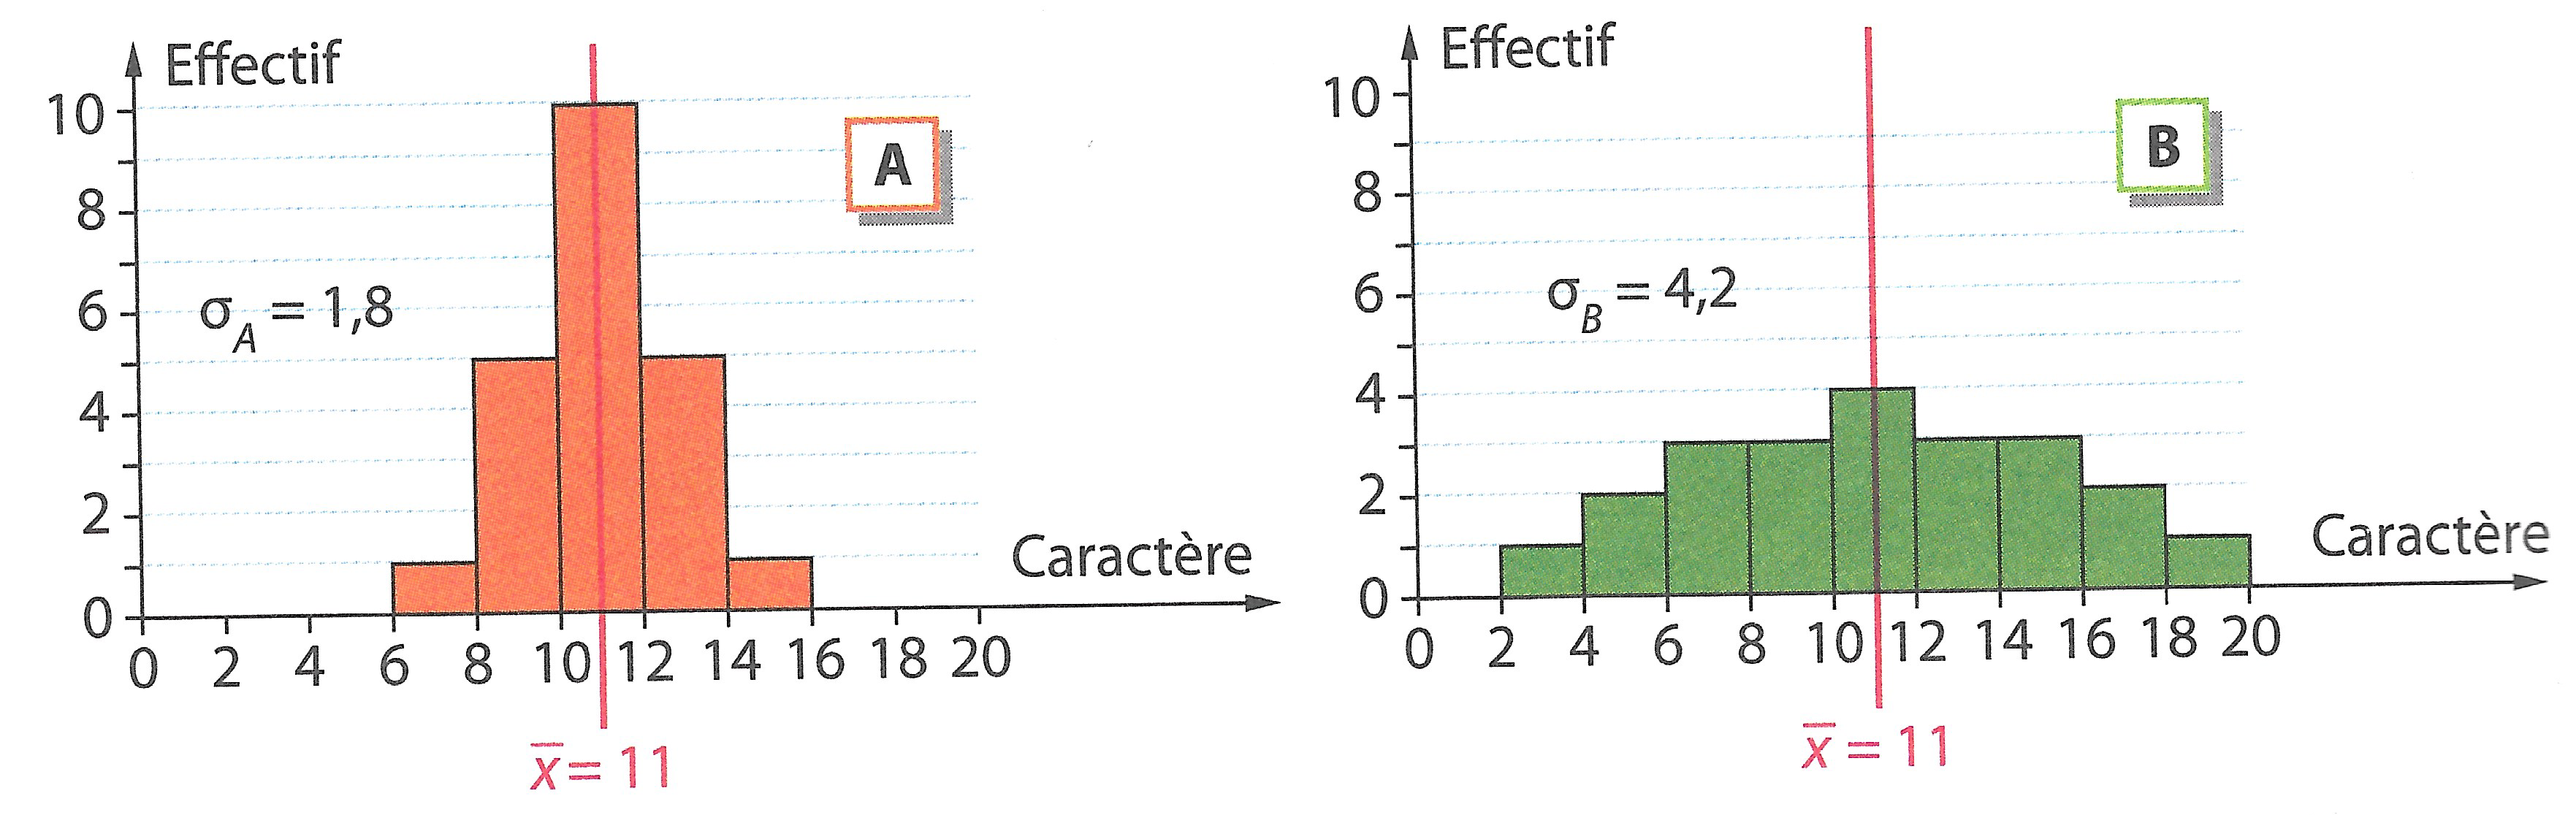
\includegraphics[scale=0.9, angle=-1.1, origin=c]{img/ex_ecart_type}
	
	$\sigma _A < \sigma _B$ : les valeurs de la série $\mathbf{B}$ sont plus dispersées que celles de la série $\mathbf{A}$ autour de $\bar{x}$. 
\end{myex}
			

\section{Diagrammes en boîte à moustaches}

\begin{mydef}
	Le \kw{diagramme en boîte à moustaches} est un dessin à l'échelle, où la <<\kw{boîte}>> est un rectangle limité par $Q_1$ et $Q_3$, et regroupe donc 50 \% des valeurs.
	
	La médiane $Me$ est repérée par un segment dans le rectangle.
	
	Le minimum $x_{min}$ et le maximum $x_{max}$ correspondent aux extrémités des <<\kw{moustaches}>>.
\end{mydef}

\begin{myex}
	Boite à moustache correspondant à l'exemple :
		\begin{center}
		 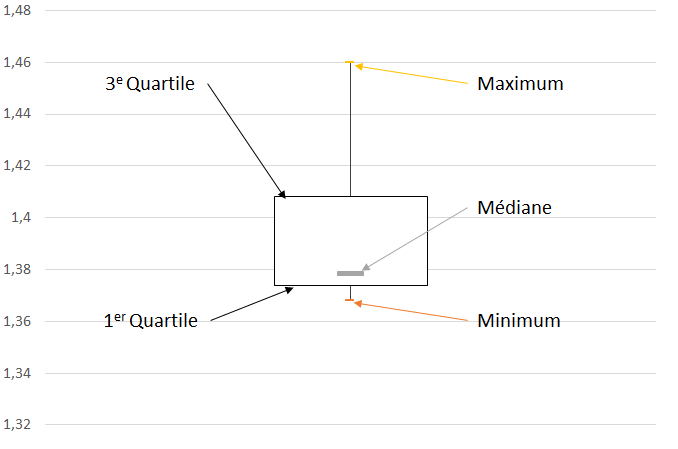
\includegraphics[scale=0.67]{img/moustache}
	\end{center}
\end{myex}
\end{document}